\section{Theory}
\fboxsep=1mm%padding thickness
\fboxrule=1pt%border thickness

\begin{figure*}[t]
    \centering
    %  trim={<left> <lower> <right> <upper>}
    %\fcolorbox{red}{yellow}{
        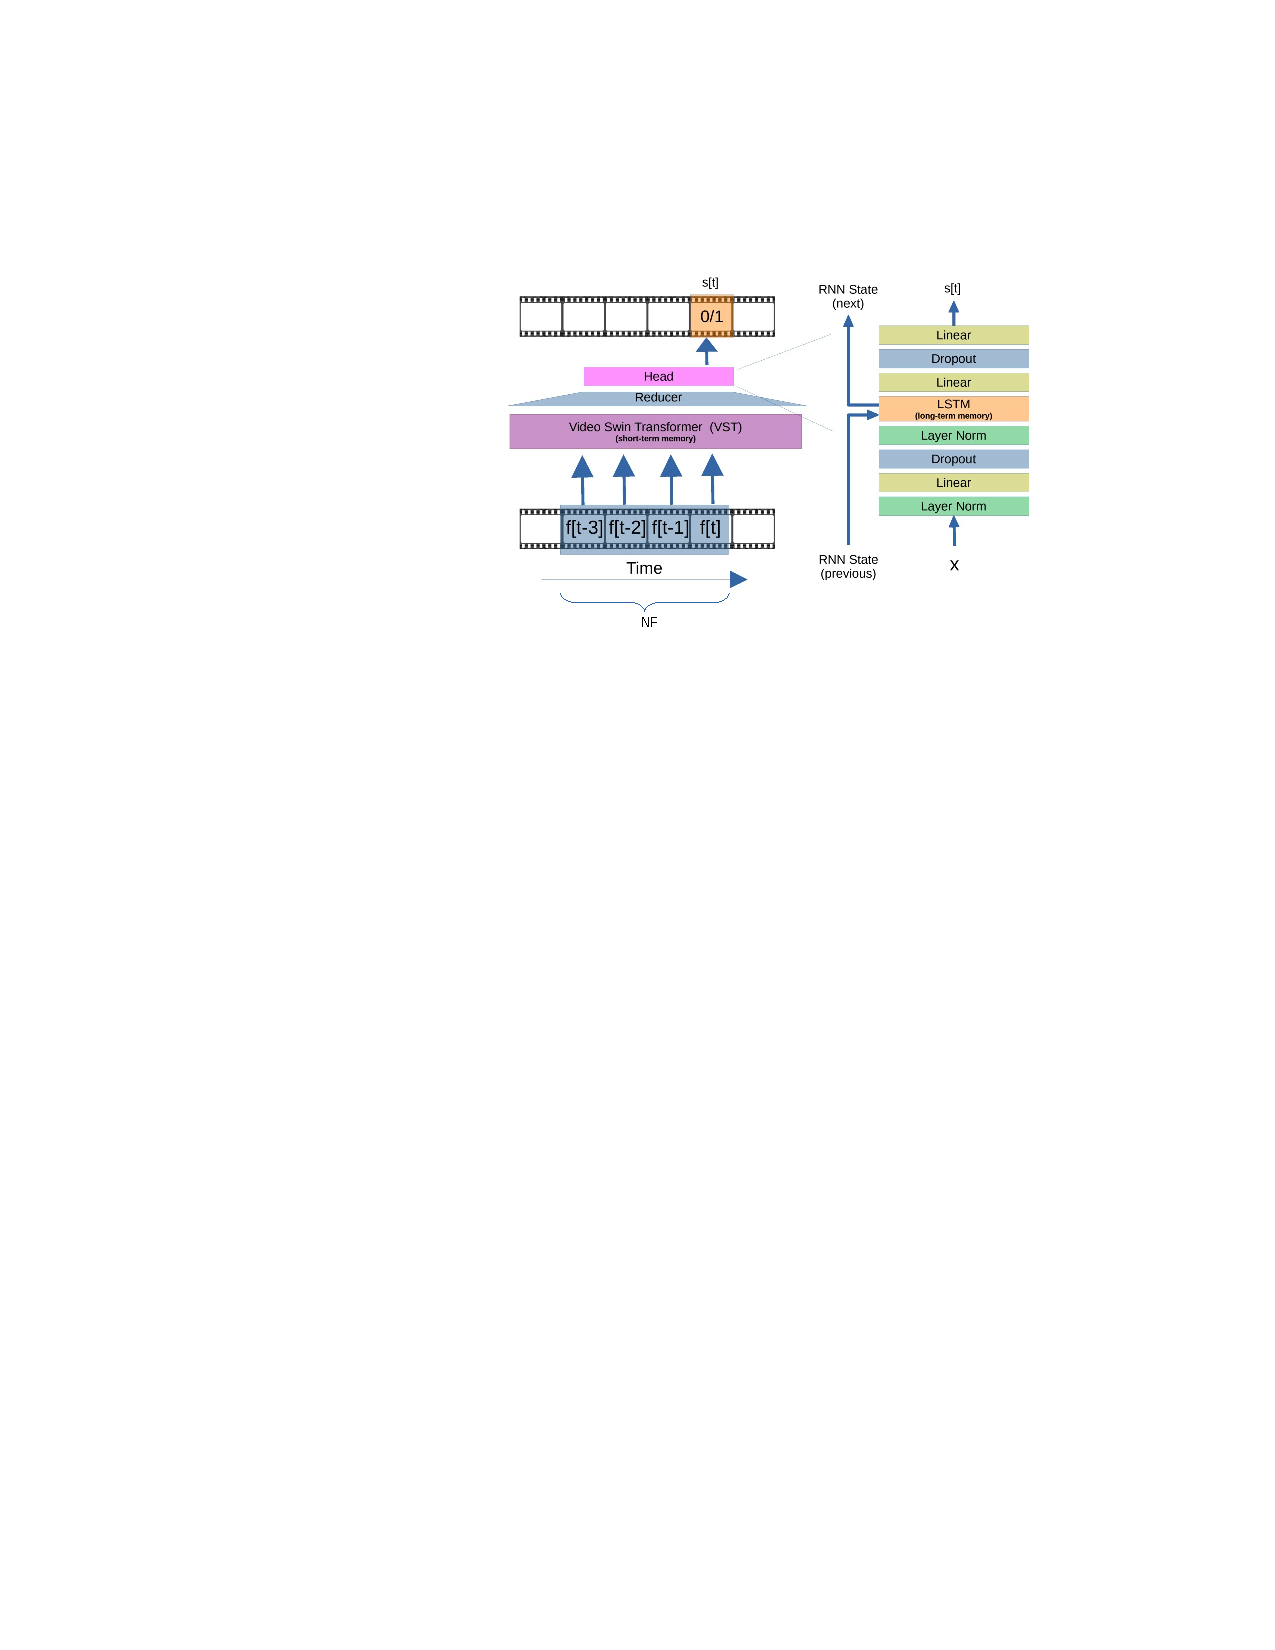
\includegraphics[trim=120 500 0 130, clip, width=1.\linewidth]{images/arch.pdf}
    %}
    % FIXME aggiungi link per immagine dei frame (copyright)
    \caption{Video frame anomaly detection architecture.}
    \label{fig:arch}
\end{figure*}

In this section, the overall architecture shown in Figure \ref{fig:arch} will be exposed.
It is composed by four main blocks: a short-term memory model to encode the information related to what is happened just now, a long-term memory model to keep track of the past, a saliency model to increase the relevant information about the scene and the final classification module, trained to classify the current frame.
% TODO descrivere la nuova annotazione ??? Check motivazioni! :)

\subsection{Short-term memory}

Since the task provides an online execution of the classification, the only information available are the current frame and the past frames.
The goal of this model is to efficiently encode the current frame and the most recent ones (last three, in this case) in the most appropriate way.
Since the frames are all available by the time they are parsed, a Transformer model is more appropriate than an RNN model due to its ability to process them in parallel.
In particular, the Video Swin Transformer (VST) \cite{liu_video_2022} was chosen as the base model due to its superior performance compared to a vanilla ViT \cite{DBLP:conf/iclr/DosovitskiyB0WZ21} model.
The VST model is the extension to video of the Swin Transformer \cite{liu2021Swin}, which is a general-purpose image backbone with high performance on tasks that involve detection and localization.
Originally born to carry out the task of video action classification, it has been adapted to detect anomalies on single frame in a near-real time fashion, considering a temporal window of the latest three frames at time $t_{i-2}$, $t_{i-1}$ and $t_{i}$.

The video extension takes in input a video with size $T \times H \times W \times 3$, where $T$, $H$ e $W$ correspond to number of frames, height width and channels RGB, respectively.
The model split the frames in non-overlapping 3D patches, partitioning the video in $\frac{T}{2} \times \frac{H}{4} \times \frac{W}{4}$ 3D tokens, projecting the features to an arbitrary dimension $C$.

\subsection{Long-term memory}

Because what happens in older frames can still be useful, there was a need for a way to keep track of the distant past.
This time the requirement is opposite to the previous one, we can only update the memory sequentially, when a new frame is available.
For this reason, our choice fell on an RNN module instead of a Transformer (LSTM in this specific case).
The hidden state $h_t$ and cell state $c_t$ encode information about the past.
In this way the model is very efficient, because it doesn't need to access the past frames again, but simply read the current state of the cell.
We have chosen to include the LSTM cell inside the classifier because the input information $x_t$ represents a summary of the information present inside the frames processed by the short-term memory model, without superfluous information.
This means that it is the ideal place to update long-term memory with new information.

\subsection{Saliency model}

\begin{figure*}[t]
    \centering
    %  trim={<left> <lower> <right> <upper>}
    %\fcolorbox{red}{yellow}{
        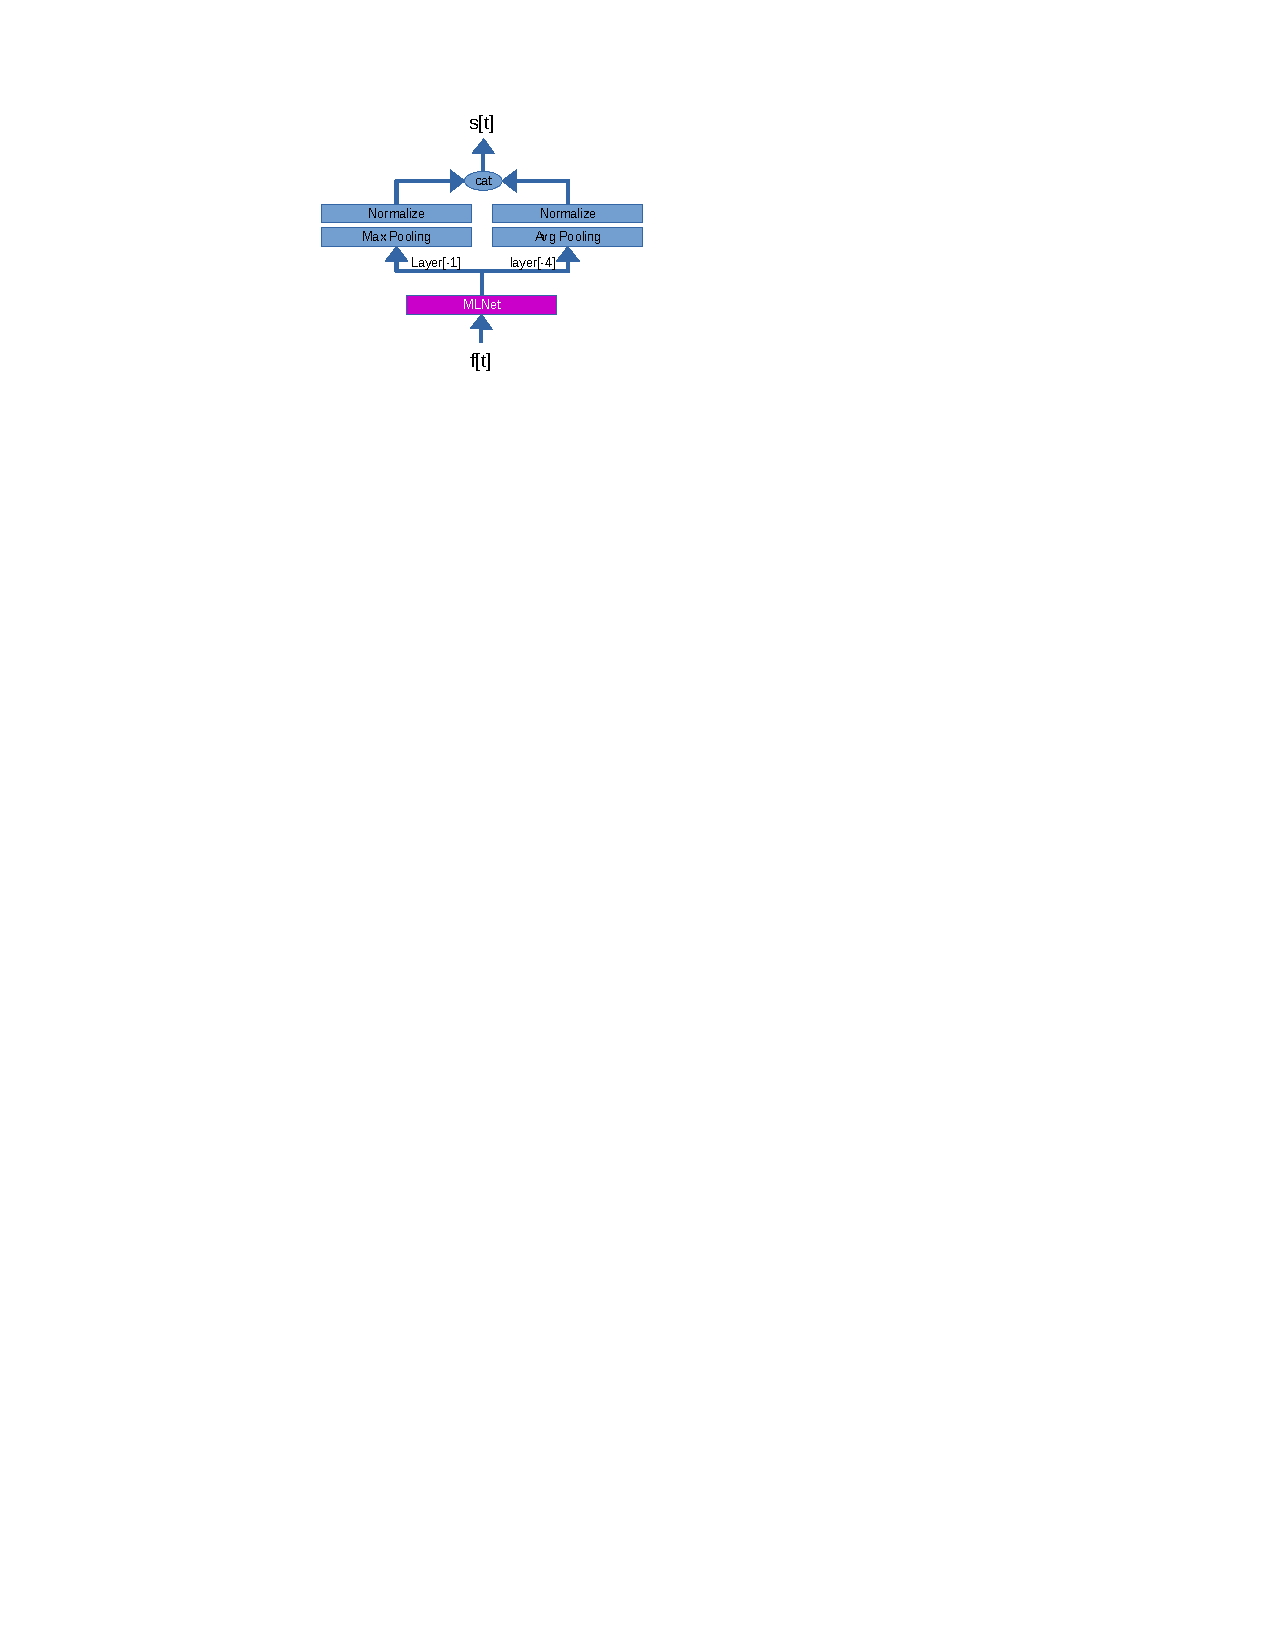
\includegraphics[trim=0 610 150 50, clip, width=1.\linewidth]{images/saliency.pdf}
    %}
    \caption{Saliency computatioon.}
    \label{fig:arch-saliency}
\end{figure*}

Taking inspiration from DRIVE \cite{bao2021drive}, we added more information about the scene present in the current frame with the help of a saliency model, used in evaluation mode.
We adopted a VGG-16-based MLNet \cite{cornia2016deep} as saliency module, pre-trained on the fixation data of the DADA-2000 \cite{fang2019dada} training set and the parameters are frozen during the training.

As seen in the Figure \ref{fig:arch-saliency}, we use the output of MLNet (last layer) and the fourth last layer.
The features are passed through a max pooling and average pooling, respectively.
Then, normalized and concatenated to form a single saliency vector $s[t]$ of 2275 values.

\subsection{Classification module}

The output is computed in the following way:

\begin{equation}
\begin{split}
    r[t_{i}] &= Reducer(VST(f[t_{i-2}], f[t_{i-1}], f[t_{i}])) \\
    o[t_{i}] &= Cls(r[t_{i}], s[t_{i-1}])
\end{split}
\end{equation}

\noindent Where $f[t_{i-2}]$, $f[t_{i-1}]$ are the buffered past frames, $f[t_{i}]$ the current frame, $r[t_{i}]$ is the output of the reducer and $o[t_{i}]$ is the classification output of the frame at time $t_{i}$, $s[t_{i-1}]$ is the LSTM state.
The output of the $VST$ is collected and the number of channels is reduced by $Reducer$ (an Adaptive Average Pool 3D) and passed to the classifier $Cls$ composed by a three fully connected layers interspersed with a LSTM cell.
The LSTM cell was introduced to maintain a relationship between frames during training.
Past memory helps the classifier find connections to past frames out of reach of the transformer.

The final output $o[t_{i}]$ is the probability of the anomaly inside the last available frame $f[t_{i}]$.
This is trained with a weighted cross-entropy loss, giving more weight to the anomaly class, because it is spotted less frequently.

The final architecture and training modality are very simple and straightforward.
The use of the Transformer allows information to be extracted in a parallel and high-performance way with respect to an LSTM, on a limited number of frames which represents our short-term memory.
While, to keep information from the distant past as a long-term memory, we introduced an LSTM network interconnected to the classifier.
The choice of introduce it into the latent space of the classifier resulted in a limited additional computational cost.

% copyright image frame: <a href="https://www.freepik.com/free-vector/realistic-vector-icon-film-tape-strip-with-white-square-isolated-white-cinema-concept_31096470.htm#query=video%20frame&position=31&from_view=keyword">Image by user15245033</a> on Freepik